
\clearpage
\JMSection{附录}

\subsection{补充材料}

\begin{enumerate}
	\item 本实验报告内容由黄罗琳、戴鹏辉共同完成,小组成员分工明确,工作任务平均。
	\item 感谢两位老师在实验中详细为我们解答每一个问题,让我们能够按时完成实验,感谢您!
	\item 相关源文件(Latex)已上传Github,相关库包含实验报告内容,如需要查看可联系我进行查阅。
\end{enumerate}
\quad \large \textbf{感谢您对于此篇实验报告的阅读与批改,祝您工作顺利!}

\subsection{原始数据与桌面}
\begin{figure}[H]
    \centering
    \begin{minipage}{0.4\textwidth} % 设置第一个图片的宽度
        \centering
        \includegraphics[width=\linewidth]{app1.jpg}
        \caption{原始数据与签名}
        \label{}
    \end{minipage}%
    \hfill
    \begin{minipage}{0.4\textwidth} % 设置第二个图片的宽度
        \centering
        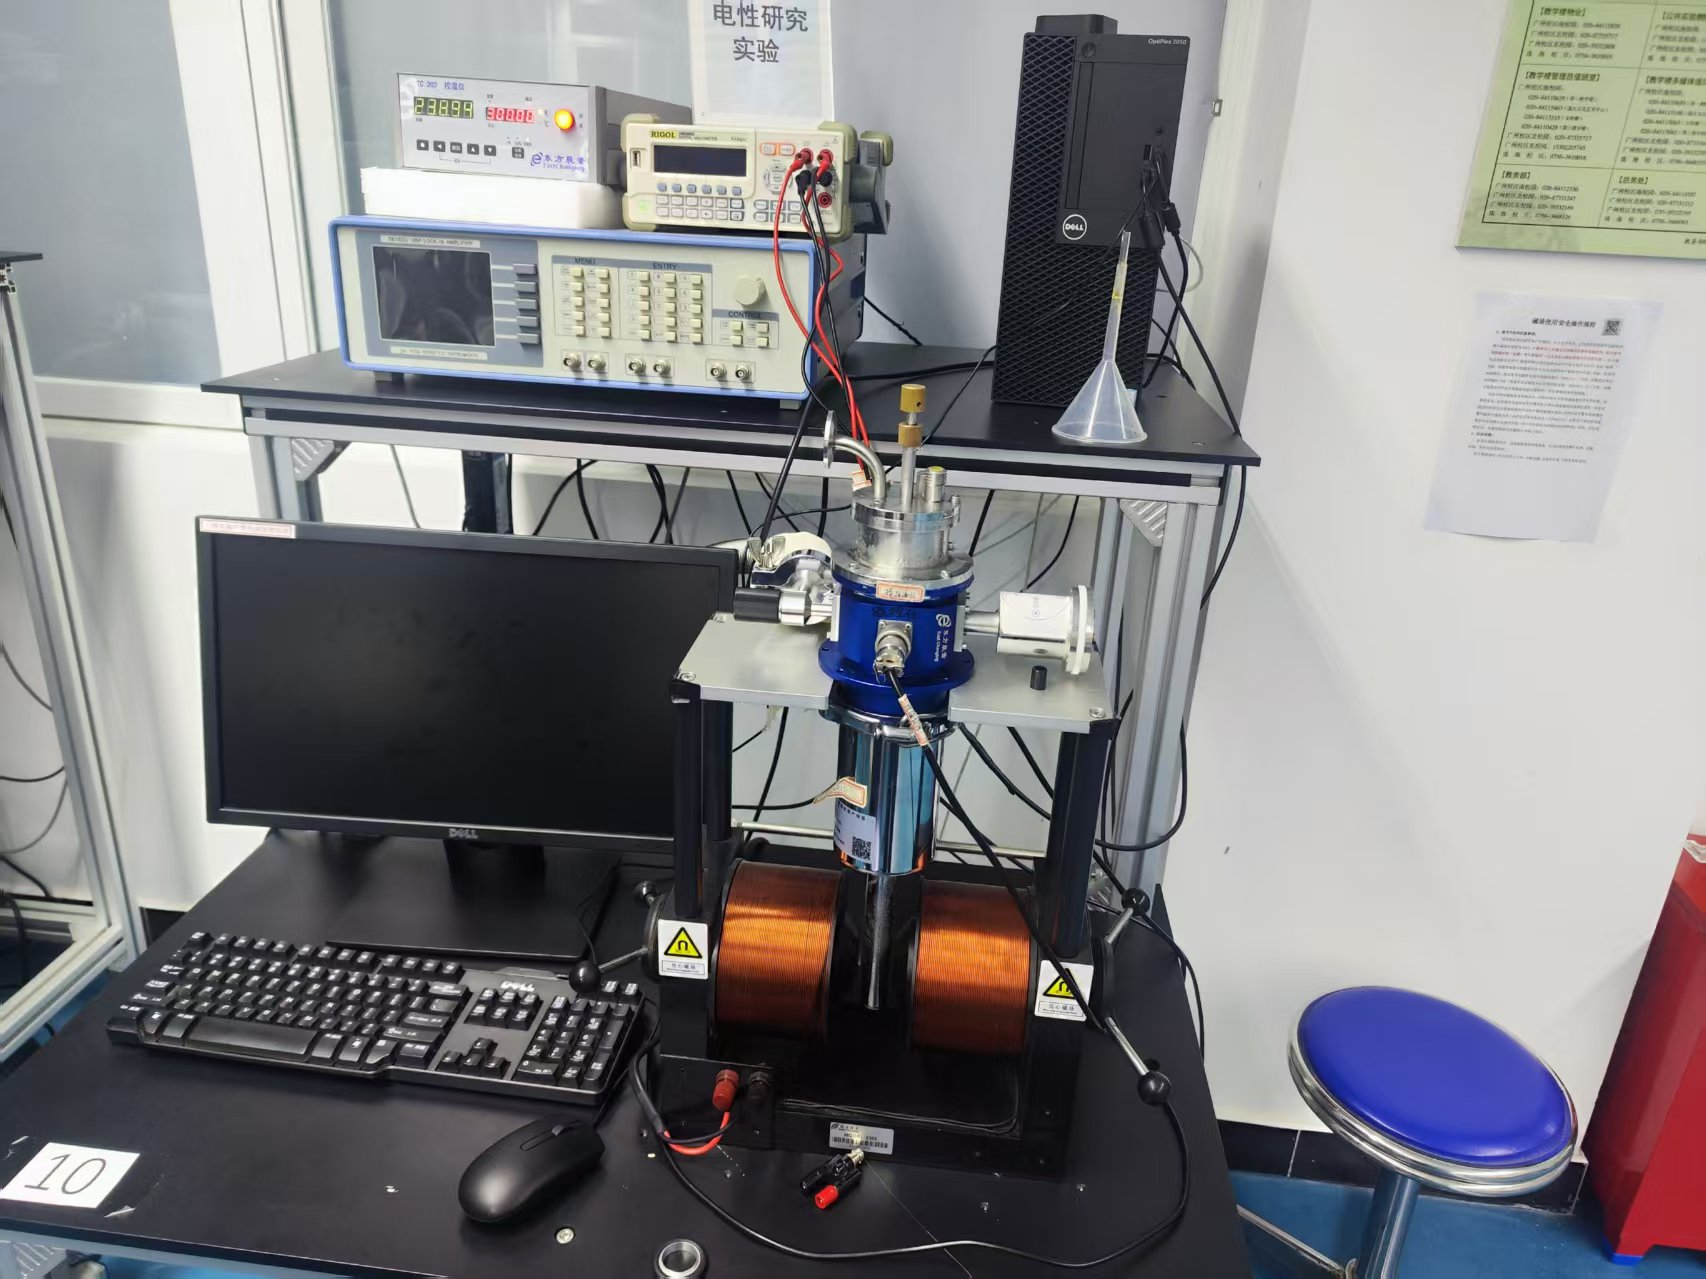
\includegraphics[width=\linewidth]{app2.jpg}
        \caption{整理后桌面}
        \label{}
    \end{minipage}
\end{figure}

\subsection{个人签名}
\begin{figure}[H]
    \centering
    \begin{minipage}{0.45\textwidth} % 第一个图片的宽度
        \centering
        \includegraphics[width=\linewidth]{签字.jpg}
        \caption{个人签名:黄罗琳}
        \label{}
    \end{minipage}%
    \hfill
    \begin{minipage}{0.45\textwidth} % 第二个图片的宽度
        \centering
        \includegraphics[width=\linewidth]{dph.jpg}
        \caption{个人签名:戴鹏辉}
        \label{}
    \end{minipage}
\end{figure}

\begin{figure}[htbp]
    \centering
    \begin{minipage}{0.7\textwidth} % 第三个图片的宽度
        \centering
        
\includegraphics[width=\linewidth]{name.png}
        \caption{个人签名:杨舒云}
        \label{fig:name}
    \end{minipage}
\end{figure}

\begin{figure}[H]
    \centering
    \begin{minipage}{0.45\textwidth} % 第四个图片的宽度
        \centering
        \includegraphics[width=\linewidth]{dhk.png}
        \caption{个人签名:丁侯凯}
        \label{}
    \end{minipage}
\end{figure}


